\documentclass{article}

\usepackage{enumerate}
\usepackage[margin=1in]{geometry}
\usepackage{amsmath, amssymb}
\usepackage{graphicx}
\usepackage[framed,numbered,autolinebreaks,useliterate]{mcode}

\newcommand{\file}[1]{\section{#1}\lstinputlisting{../#1}}

\begin{document}

\title{18-758 Project Report}
\author{Jean-Baptiste Cordonnier - Thomas Mullins}
\date{\today}
\maketitle


\section{Pulse}

We use a square-root raised cosine pulse with a rolloff factor of $\alpha =
0.25$. The pulse was chosen because it is a Nyquist pulse of unit energy, which
minimizes ISI, and because it conveniently falls off quickly in both the time
domain and in the frequency domain.

\[
  \text{SRRC}(t) = \left\{
    \def\arraystretch{3.2}
    \begin{array}{lr}
      \dfrac{1 - \alpha + \frac{4}{\pi}\alpha}{\sqrt{T_s}} & t = 0 \\
      \dfrac{\alpha \left(
        \left(1 + \frac{2}{\pi}\right) \sin{\frac{\pi}{4\alpha}} +
        \left(1 - \frac{2}{\pi}\right) \cos{\frac{\pi}{4\alpha}}
      \right)}{\sqrt{2T_s}} & |t| = \frac{T_s}{4\alpha} \\
      \dfrac{
        \sin{\left((1-\alpha)\frac{\pi}{T_s}t\right)} +
        \frac{4\alpha}{T_s}t\cos{\left((1+\alpha)\frac{\pi}{T_s}t\right)}
      }{
        \frac{\pi}{\sqrt{T_s}}t
        \left(1-\left(\frac{4\alpha}{T_s}t\right)^2\right)
      } & otherwise
    \end{array}
  \right.
\]

$T_s = 8$\textmu s is the symbol period for our transmitted signal. When
sampling the received signal, we use a matched filter to optimally boost the
signal while suppressing noise.

\section{Frequency sync}

We do not do frequency synchronization in the final version of our project. We
found that the periodic channel re-estimation is sufficient to handle the
gradual phase drift.

Initially we had a string of 40 ones at the start of the packet, and then the
receiver would search for a peak in the discrete fourier transform of the
starting sequence and apply a correction to the whole received signal. However,
this was ineffective because of the wildly fluctuating phase at the start of the
signal, which can be seen in figure~\ref{fig:phase}. Next we tried throwing out
the first 250\textmu s or so of the received signal and putting the frequency
synchronization sequence after that, where the phase has a linear drift. This
worked better, but it was then too hard to fit the entire message into
800\textmu s, so we removed frequency synchronization altogether.

\begin{figure}
  \centering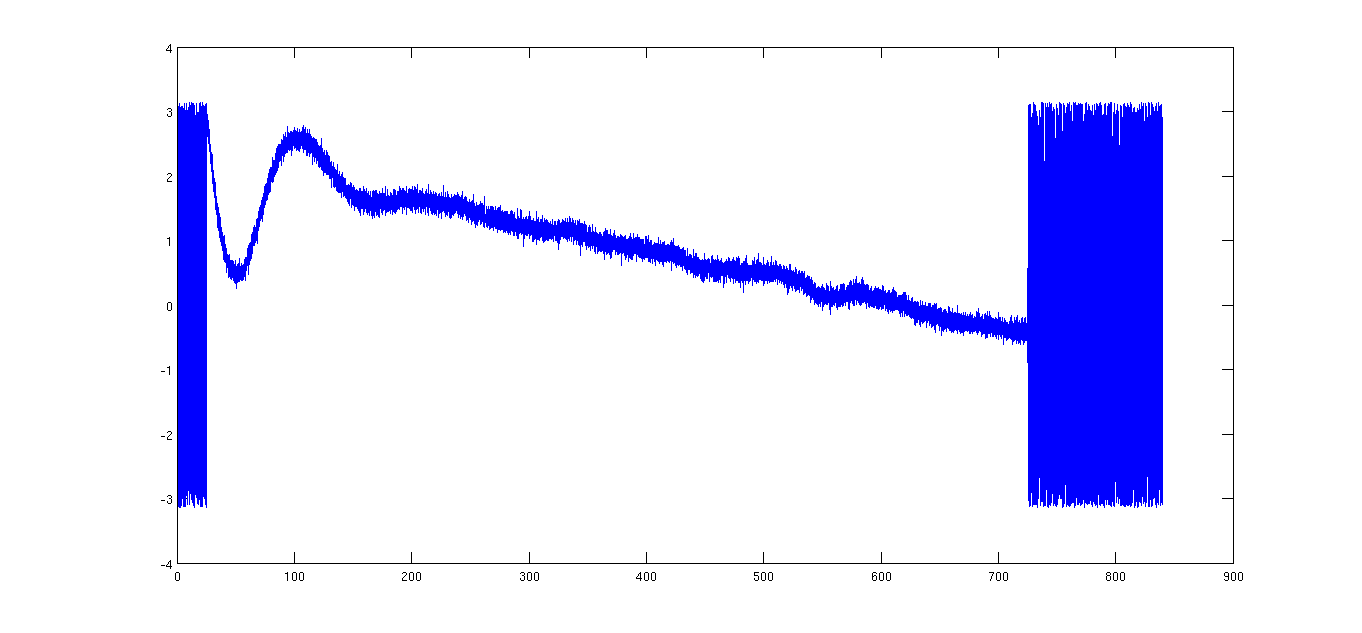
\includegraphics[width=\textwidth]{../presentation/phase.png}
  \caption{Received phase when sending all ones}
  \label{fig:phase}
\end{figure}

\section{Timing sync}

We use a simplified version of the timing synchronization we have seen in class. We use a random sequence of symbols that is highly uncorrelated, such that we see a high peak during the correlation of the message and the timing synchronization (see plot). Then we get $\hat\tau$ and know where the signal starts exactly. 

% Todo correlation plot

\section{One-tap equalizer}

We are using a one-tap equalizer for each segment of the message. We send 5-length symbols pilot every 120 symbols of information. The one tap equalizer uses the following formula :

\[
  h_0 = \frac{\text{txPilot} \cdot \text{rxPilot}}{\text{txPilot}^2}
  \hspace{2cm}
  \text{eqMessage} = \frac{\text{message}}{h_0}
\]

The equalization is very efficient as we can see on the following plot. Even if the pilot sequence is very short, the $h_0$ is still precise and equalize well the received segment of the message. It corrects the phase drift and the modulus of the signal. 

% Todo equalizer plot

\section{Constellation}

We are using a 4-PSK constelation. 

\begin{figure}
  \centering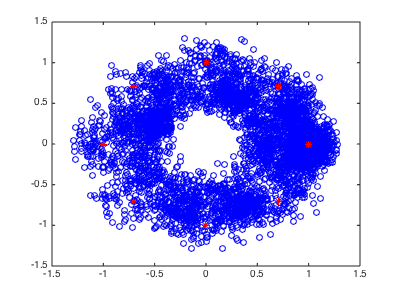
\includegraphics[width=\textwidth]{../presentation/8psk.png}
  \caption{Received symbols when using 8-PSK}
  \label{fig:8psk}
\end{figure}

\begin{figure}
  \centering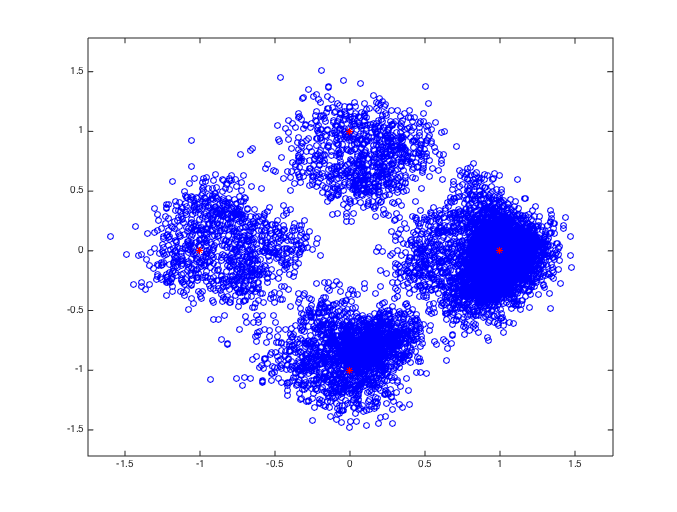
\includegraphics[width=\textwidth]{../presentation/4psk.png}
  \caption{Received symbols when using 4-PSK}
  \label{fig:4psk}
\end{figure}

\section{Channel Coding}

We are using a rate $\frac{3}{4}$, 64 state convolutional code. The matrix
which describes the trellis was taken from the lecture handouts:

\[
  g =
  \begin{pmatrix}
    6 & 1 & 4 & 3 \\
    3 & 4 & 0 & 7 \\
    2 & 6 & 7 & 1
  \end{pmatrix}
\]

In this matrix $g$, each row corresponds to an information bit, each column
corresponds to a coded bit, and each element is an octal number whose binary
representation describes which bits of history are exclusive-or'd together. Each
row has elements up to three bits in size for a total of nine input bits. Of
these, six are state bits and three are new information bits. This means there
are a total of 64 states in the trellis.

Before encoding, $(\nu+1) \cdot 3 = 21$ zeros are appended to the signal so that
it always ends in a known state, which improves the error rate of the last few
information bits. If this is not done, the last few bits do not have the full
benefit of the convolutional code.

The receiver uses hard decoding on received symbols to recover the coded bits,
and then uses the Viterbi algorithm to recover the information bits. Hard
decoding is done using a standard minimum distance detector. Viterbi decoding
involves first walking forward through the trellis, calculating the minimum
cumulative bit error for each branch entering a state and keeping track of which
branch that minimum is from. Then the decoder walks backwards through the
trellis, following the path of minimum bit error, and recording the information
bits which produce that path.

The channel coding is effective, but could much more effective if we used a
lower rate convolutional code. With a couple bit errors very near each other,
the rate $\frac{3}{4}$ code can amplify the error and cause a larger string of
errors, which is occasionally a problem. Also, as seen in figure~\ref{fig:pics}
there is always a string of errors near the end. This could be some noise that
always appears near the end of the image, such as due to the drifting phase of
the signal. This could also be due to a bug in the Viterbi decoding.
Interleaving may help alleviate some of these problems.

\section{Conclusion}

% TODO add some more images of received signals

\begin{figure}
  % TODO final images
  %\centering\includegraphics[width=\textwidth]{}
  \caption{Transmitted and Received Images}
  \label{fig:pics}
\end{figure}


\clearpage
\appendix
\file{params.m}
\file{receiver.m}
\file{transmitter.m}
\file{doTimingSync.m}
\file{doSampling.m}
\file{srrc.m}
\file{applyPulse.m}
\file{channelEncode.m}
\file{channelDecode.m}
\file{plotSignal.m}
\file{DTFT.m}

\end{document}
